\documentclass[conference]{IEEEtran}
\IEEEoverridecommandlockouts

\usepackage{cite}
\usepackage{amsmath,amssymb,amsfonts}
\usepackage{algorithmic}
\usepackage{graphicx}
\usepackage{textcomp}
\usepackage{xcolor}
\usepackage{tikz}
\usepackage{algorithm}

\usetikzlibrary{arrows.meta, positioning, shapes.geometric}

\begin{document}

\title{ML-Based Task Assignment and Deadline Prediction for Agile Project Management with Automated Workflow Integration}

\author{
\IEEEauthorblockN{Muhammad Risyad Himawan Putra}
\IEEEauthorblockA{
Department of Informatics\\
Institut Teknologi Sepuluh Nopember\\
Surabaya, Indonesia\\
5025231205@student.its.ac.id
}
\and
\IEEEauthorblockN{Riyanarto Sarno}
\IEEEauthorblockA{
Department of Informatics\\
Institut Teknologi Sepuluh Nopember\\
Surabaya, Indonesia\\
riyanarto@its.ac.id
}
\and
\IEEEauthorblockN{Kurnia Cahya Febryanto}
\IEEEauthorblockA{
Department of Informatics\\
Institut Teknologi Sepuluh Nopember\\
Surabaya, Indonesia\\
6025241065@student.its.ac.id
}
}


\maketitle

\begin{abstract}
Agile and Scrum teams frequently face operational challenges such as inconsistent task assignment, uncertain deadline estimation, and high manual overhead during sprint execution. This study investigates the feasibility of integrating machine learning–based predictions into automated Agile workflows to support task assignment and deadline estimation. Using the AgileScrumSprintVelocityDataSet, an XGBoost-based classifier is employed for assignee recommendation, while regression models are examined for completion-time estimation using Jira like issue metadata. After hyperparameter tuning, the assignee model achieves a Top-1 accuracy of 78.79\% and a Top-3 accuracy of 94.55\% on the evaluated dataset. For deadline prediction, the selected regression model attains a mean absolute error of 0.92 days, a mean absolute percentage error of 6.84\%, and an $R^2$ score of 0.435, indicating low absolute error despite modest explained variance. The models are deployed as RESTful services and embedded into an n8n-orchestrated workflow to enable automated field updates and periodic re-evaluation during active sprints. These results demonstrate the practical feasibility of operationalizing machine learning models within workflow automation, while highlighting the inherent limitations of deadline prediction in complex Agile project environments.
\end{abstract}

\begin{IEEEkeywords}
Agile Software Development, Deadline Prediction, Machine Learning, Task Assignment, Workflow Automation
\end{IEEEkeywords}


\section{Introduction}

Agile and Scrum have become dominant approaches for managing modern software projects due to their iterative delivery, rapid feedback cycles, and adaptability to changing requirements. Empirical evidence suggests Scrum is widely practiced: a large-scale literature review reports that by 2021, Scrum or hybrid variants were used by the majority of surveyed organizations \cite{verwijs2023_scrum}. Empirical comparisons also indicate that agile and hybrid approaches can improve stakeholder success compared to purely traditional approaches \cite{gemino2021_project_success}. These trends highlight why data-driven support for sprint execution and decision-making is increasingly relevant in agile environments.

Despite wide adoption, Agile/Scrum teams still frequently face recurring operational problems, particularly sprint delays, rework, and workload imbalance. These issues are intensified by high coordination and monitoring demands: evidence from large-scale analytics data on IT professionals shows working hours can increase by about 30\% and measured productivity can decline in the 8--19\% range under higher coordination friction \cite{gibbs2023_wfh_productivity}. Workload distribution and role clarity also matter for sustainability, a field study of 1,894 developers across 217 project teams shows agile method use is associated with reduced work exhaustion through clearer role perceptions \cite{venkatesh2020_work_exhaustion}. In practice, project decision-making (assignment, due dates, and follow-ups) is still often handled manually or via ad-hoc conventions, which can amplify delays and inconsistent task handling under sprint pressure.

A key limitation of current project management automation is its predominantly rule-based and static nature, which limits adaptability to evolving and noisy project contexts \cite{prinz2021_lowcode_slr, zhao2021_trigger_action}. While prior research has demonstrated the effectiveness of machine learning for issue assignment and resolution-time prediction \cite{diamantopoulos2023_issue_assignment, sousa2023_task_effort, nastos2025_resolution_time}, many existing approaches remain disconnected from operational workflows and are evaluated in an offline setting \cite{mahdi2021_spm_slr, cabral2023_ensemble_effort}. As a result, prediction outputs typically do not trigger automated actions or continuous re-evaluation during sprint execution \cite{prinz2021_lowcode_slr, yasmin2024_airflow_wac}. This gap motivates the need for architectures that operationalize machine learning models as real-time decision services embedded within workflow orchestration systems.

Therefore, this study proposes an integrated architecture that operationalizes ML predictions directly inside an n8n-orchestrated Agile workflow via a Flask REST API (XGBoost-based assignee recommendation and a lightweight regression-based deadline estimator). This study is guided by the following research objectives:
(O1) To evaluate the predictive capability of Jira like issue metadata for assignee recommendation and deadline estimation using supervised learning models.
(O2) To analyze the impact of embedding machine learning predictions into an automated workflow on the consistency of task updates during sprint execution.
(O3) To assess the effectiveness of periodic re-evaluation mechanisms in maintaining prediction relevance for incomplete or returned issues within active sprints.

The main contributions of this work are as follows:
\begin{itemize}
    \item An empirical evaluation of machine learning models for assignee recommendation and deadline estimation using real-world Agile project data.
    \item A workflow-aware integration of predictive models into an automated Agile pipeline, enabling continuous execution and re-evaluation within active sprints.
    \item An analysis of periodic re-prediction strategies for handling incomplete or reverted issues, examining their robustness compared to single-shot offline prediction.
\end{itemize}




\begin{table*}[t]
\caption{Gap Analysis of Recent Work and the Positioning of This Study}
\centering
\renewcommand{\arraystretch}{1.25}
\begin{tabular}{p{3.2cm} p{4.0cm} p{4.5cm} p{5.0cm}}
\hline
\textbf{Study} & \textbf{Approach} & \textbf{Limitation} & \textbf{Gap Addressed by This Work} \\
\hline
Shamim et al. \cite{shamim2025_costreview} &
Review of AI for cost/effort estimation &
Model-centric; limited discussion on operational workflow embedding &
Deployable ML services integrated into workflow engine for real-time execution \\

Sousa et al. \cite{sousa2023_task_effort} &
ML for task effort/duration estimation &
Standalone predictor; not integrated into automation loop &
Predictions trigger automated updates and periodic re-evaluation during sprint \\

Prinz et al. \cite{prinz2021_lowcode_slr} &
Low-code platform literature review &
Automation often rule-based; brittle with evolving contexts &
ML-driven predictions adapt workflows beyond static rules \\

Gupta et al. \cite{gupta2023_action_suggestions} &
Intelligent assistance for low-code automation authoring &
Focus on recommending next actions, not project decision prediction &
Uses ML to predict project decisions (assignee/deadline) and execute actions \\

Yasmin et al. \cite{yasmin2024_airflow_wac} &
Workflows-as-code challenges (Airflow case study) &
Focus on pipeline orchestration challenges; not project-ticket automation &
Applies orchestration concepts to Agile tickets with ML decision support \\

P\'erez Castillo et al. \cite{perezcastillo2024_sprint_velocity} &
Sprint progress/velocity evaluation with ML &
Sprint analytics; limited automation into issue operations &
Operationalizes sprint monitoring via scheduled re-check and automated updates \\

Diamantopoulos et al. \cite{diamantopoulos2023_issue_assignment} &
Automated issue assignment via topic modeling &
Assignment recommendation without end-to-end workflow enforcement &
End-to-end pipeline: prediction $\rightarrow$ update fields $\rightarrow$ notify $\rightarrow$ re-check \\

Choetkiertikul et al. \cite{choetkiertikul2025_sprint2vec} &
Sprint representation learning (Sprint2Vec) &
Emphasis on characterization; integration into tooling not central &
Uses lightweight predictors integrated into workflow actions for practical adoption \\

\textbf{Proposed Method} &
\textbf{Supervised ML for assignee and deadline prediction integrated into n8n workflow orchestration} &
\textbf{Focus on operational feasibility; predictive performance limited by available issue metadata} &
\textbf{Empirical evaluation and workflow-aware integration enabling real-time updates and periodic re-evaluation} \\

\hline
\end{tabular}
\label{table:gap}
\end{table*}

% -------------------------------------------------------------
\section{Related Work}
% -------------------------------------------------------------

This section reviews related work on machine learning for software project management, workflow automation, Agile sprint prediction, and task assignment, and concludes by identifying the research gaps addressed in this study.

% -------------------------------------------------------------
\subsection{Machine Learning for Software Project Management}

Machine learning (ML) has been widely applied to support software project management decisions, particularly in cost and effort estimation, schedule prediction, and risk assessment. Systematic literature reviews consistently report that supervised learning and ensemble approaches outperform traditional statistical baselines, although many studies remain offline and context-dependent, limiting their operational adoption \cite{shamim2025_costreview, mahdi2021_spm_slr}. Recent work has also emphasized best practices for effort estimation models, including feature stability, cross-project generalization, and rigorous evaluation protocols \cite{brar2022_effort_slr, cabral2023_ensemble_effort}.

Beyond effort estimation, ML-based prediction of task effort and duration using issue-level metadata has shown that reliable estimates can be obtained from lightweight features suitable for integration into project tools \cite{sousa2023_task_effort}. Parallel research has explored software project risk prediction using modern ML pipelines, but these studies often prioritize predictive accuracy over deployable integration patterns for real-time workflows \cite{mahmud2022_risk_slr}. In addition, recent AutoML frameworks have been proposed to automate feature selection, model configuration, and evaluation for software project analytics, providing end-to-end modeling pipelines \cite{automl_se_slr}. However, these approaches primarily focus on offline optimization and benchmarking, and rarely address integration into live project workflows or automated execution environments \cite{automl_se_slr, prinz2021_lowcode_slr, yasmin2024_airflow_wac}.



% -------------------------------------------------------------
\subsection{Workflow Automation in Software Development}
% -------------------------------------------------------------

Workflow automation platforms enable teams to orchestrate triggers, transformations, and actions across heterogeneous tools such as issue trackers, repositories, and notification systems. Research on low-code and end-user automation shows that such platforms reduce development effort and accelerate automation creation, but workflows are predominantly rule-based and can become brittle under evolving project contexts \cite{prinz2021_lowcode_slr}. Recent studies have explored intelligent assistance for automation authoring, including personalized next-action recommendations and trigger-action synthesis from natural language, highlighting opportunities for augmenting automation design with machine learning \cite{gupta2023_action_suggestions, yusuf2022_tap_generation}. In parallel, workflows-as-code approaches improve reproducibility and monitoring in pipeline orchestration, yet developers continue to report challenges in configuration and integration with external systems \cite{yasmin2024_airflow_wac}. Despite these advances, direct integration of predictive ML services into operational project workflows remains limited, with most automation focusing on static rules rather than data-driven decision updates.


% -------------------------------------------------------------
\subsection{Agile Sprint Prediction and Planning}
% -------------------------------------------------------------

Agile sprint planning relies on accurate estimation and forecasting of sprint outcomes such as velocity, progress, and completion risk. Prior work has explored machine learning models for sprint progress and velocity evaluation using structured sprint artifacts, demonstrating the predictive potential of historical sprint data \cite{perezcastillo2024_sprint_velocity}. Complementary research has investigated sprint characterization and representation learning to capture sprint dynamics for forecasting and retrospective analysis \cite{choetkiertikul2025_sprint2vec}. At both sprint and issue levels, supervised regression and NLP-enhanced models have been applied to effort and story-point estimation, improving planning inputs from textual and metadata features \cite{ramessur2021_sprint_effort, yalciner2024_storypoint_sbert}. However, most sprint prediction studies evaluate models as standalone predictors rather than embedding them into automated operational workflows.

% -------------------------------------------------------------
\subsection{Task Assignment and Resource Allocation}
% -------------------------------------------------------------

Task assignment and resource allocation have been studied via developer recommendation and optimization-based workload balancing. For issue assignment, topic-modeling and semantic feature extraction from Jira issue tracking data has been shown to enable automated assignment recommendations, though the focus is often on modeling accuracy rather than closed-loop workflow execution \cite{diamantopoulos2023_issue_assignment}. In bug triage and developer recommendation, deep learning and multimodal ensemble techniques improve assignment quality by modeling developer activity and heterogeneous signals \cite{guo2020_bug_triage, zhang2023_susrec}.

For resource allocation, optimization-based approaches (e.g., goal programming) have been used to allocate resources under constraints in agile-based development contexts, while reinforcement learning has been increasingly explored for resource-constrained project scheduling \cite{kaur2023_agile_resource_alloc, cai2024_drl_rcpsp}. Nevertheless, the integration of (i) ML-driven assignment and deadline prediction with (ii) automated workflow engines that continuously re-evaluate sprint tasks remains underexplored.

% -------------------------------------------------------------
\subsection{Research Gap Analysis}

Across the reviewed literature, three consistent gaps emerge: most machine learning studies for software project management remain offline and do not operationalize predictions within active project workflows; workflow automation research predominantly emphasizes rule-based execution or authoring assistance rather than predictive decision services; and task assignment, sprint prediction, and deadline estimation are typically treated as isolated problems without unified orchestration across the sprint lifecycle. This work addresses these gaps by empirically evaluating supervised ML models for assignee recommendation and deadline estimation and integrating them into an n8n-orchestrated workflow that supports real-time field updates, periodic re-evaluation, and continuous monitoring during Agile execution.


\begin{figure*}[t]
\centering
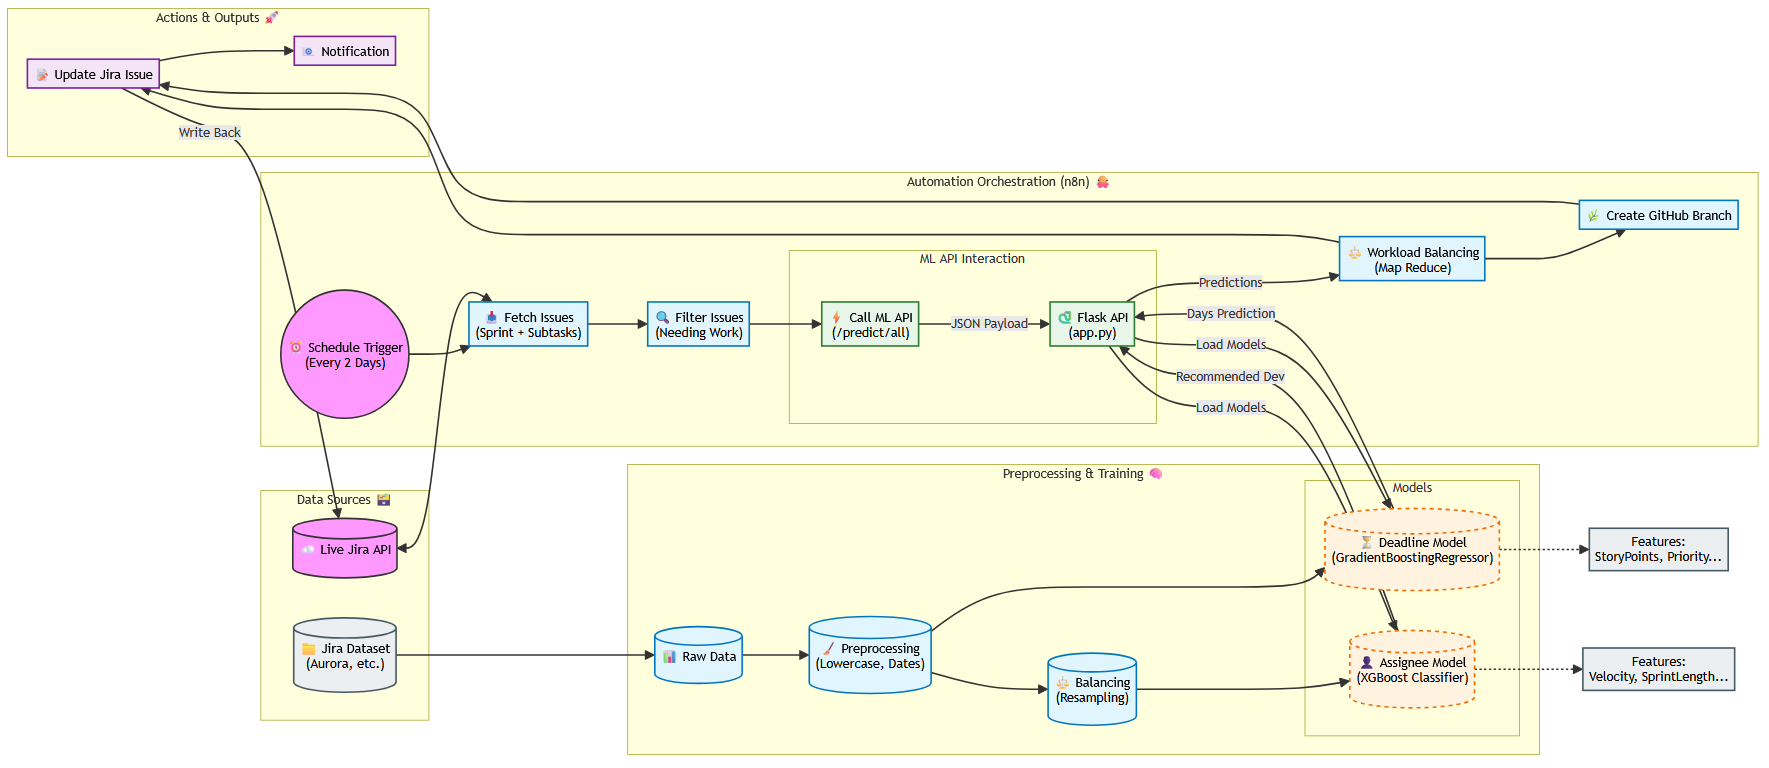
\includegraphics[width=\textwidth]{figures/system_flow.png}
\caption{Overall system architecture integrating dataset processing, machine learning models, API services, and n8n-based workflow automation.}
\label{fig:systemflow}
\end{figure*}


% -------------------------------------------------------------
% -------------------------------------------------------------
% -------------------------------------------------------------
\section{Proposed Method}
% -------------------------------------------------------------

This section presents the proposed end-to-end architecture for intelligent Agile workflow automation, as illustrated in Fig.~\ref{fig:systemflow}.

The proposed method prioritizes operational feasibility under real-world Agile automation constraints, including limited feature availability, class imbalance, and low-latency inference requirements. Model choices and configurations are therefore guided by empirical benchmarking and deployment considerations rather than algorithmic novelty.

% -------------------------------------------------------------
\subsection{Dataset Description and Preprocessing}
% -------------------------------------------------------------

\subsubsection{Dataset Source and Characteristics}
The primary dataset is the AgileScrumSprintVelocityDataSet~\cite{koralage2023_velocity}, which provides Jira like issue metadata, sprint logs, and resolution-time attributes across multiple open-source projects. In this work, the assignee classifier is trained on the Aurora subset due to its complete assignee labels, while the deadline model is trained on a merged multi-project subset to improve generalization.

\subsubsection{Dataset Statistics}
Table~\ref{tab:dataset_stats} summarizes the key dataset splits used in this study (raw merge, filtered for valid assignees, and balanced training set for the multi-class assignee model).

\begin{table}[t]
\centering
\caption{Dataset statistics used in this study.}
\renewcommand{\arraystretch}{1.15}
\begin{tabular}{l c}
\hline
\textbf{Subset} & \textbf{\#Records} \\
\hline
Aurora merged (issues+summary+sprints) & 910 \\
Aurora after dropping empty assignee & 861 \\
Aurora after whitelist filtering (8 devs) & 824 \\
Aurora balanced set (oversampling-only) & 2104 \\
Merged multi-project set (deadline model) & (varies) \\
\hline
\end{tabular}
\label{tab:dataset_stats}
\end{table}

\subsubsection{Cleaning, Encoding, and Normalization}
Each issue record is converted into a structured feature vector. Categorical fields (e.g., issue type, status, project) are encoded via one-hot encoding. Missing values are handled using simple imputation, while categorical features are encoded using one-hot encoding; scaling is only applied during benchmarking for models that require normalized inputs (e.g., SVM or linear regression).

\subsubsection{Feature Engineering}
Issue records are represented using a hybrid feature set that combines (i) lightweight structured metadata and (ii) textual content. Specifically, numeric features include story points and priority ID, categorical fields (issue type, project, and status) are one-hot encoded, and a text field (\textit{text\_content}) is vectorized using TF--IDF with a fixed vocabulary size (max\_features=500) and English stop-word removal. This design captures both ticket semantics and operational context while remaining compatible with low-latency inference in automation. The text feature is constructed by concatenating the issue summary and description fields, reflecting the information available to developers during issue creation. 

% -------------------------------------------------------------
\subsection{Machine Learning Models}
% -------------------------------------------------------------

\subsubsection{Task Assignment Model (XGBoost Classifier)}
Task assignment is formulated as a multi-class classification problem. For each issue feature vector $\mathbf{x}_i$, the model predicts an assignee class $y_i \in \{1,\dots,K\}$. XGBoost learns an additive ensemble of trees:
\begin{equation}
\hat{\mathbf{p}}_i = \mathrm{softmax}\Big(\sum_{t=1}^{T} f_t(\mathbf{x}_i)\Big),
\label{eq:xgb_pred}
\end{equation}
where $f_t(\cdot)$ is the $t$-th tree and $\hat{\mathbf{p}}_i$ is the predicted class-probability vector.

The objective minimized by XGBoost is:
\begin{equation}
\mathcal{L} = \sum_{i=1}^{N} \ell\big(y_i,\hat{\mathbf{p}}_i\big) + \sum_{t=1}^{T}\Omega(f_t),
\label{eq:xgb_obj}
\end{equation}
where $\ell(\cdot)$ is the multiclass log-loss and $\Omega(\cdot)$ regularizes tree complexity.

\begin{table}[t]
\centering
\caption{Assignee model: features and key hyperparameters.}
\renewcommand{\arraystretch}{1.15}
\begin{tabular}{l l}
\hline
\textbf{Item} & \textbf{Value} \\
\hline
Model & XGBoost multi-class classifier \\
Main features & story points, priority, sprint velocity, \\
& sprint length, completed SP, dev count, \\
& issue type, status, project, task label \\
n\_estimators & 400 \\
max\_depth & 10 \\
learning\_rate & 0.05 \\
subsample / colsample & 0.8 / 0.8 \\
eval metric & mlogloss \\
Output & top-1 + top-$k$ recommendations \\
\hline
\end{tabular}
\label{tab:xgb_config}
\end{table}

Hyperparameters such as the number of trees and maximum depth were selected using grid-search cross-validation on the training data, optimizing validation accuracy while controlling overfitting and inference latency.

\subsubsection{Deadline Prediction Model (Random Forest Regressor)}
Deadline estimation is formulated as regression of completion duration (in days). A Random Forest regressor is used due to its robustness on heterogeneous tabular features and stable inference behavior. The model uses compact issue-time features derived from story points: \textit{storypoint}, \textit{points\_per\_issue}, and a simple \textit{complexity} proxy. In the dataset, \textit{points\_per\_issue} is computed at the sprint level as the ratio between sprint story points and the number of issues, while \textit{complexity} is defined as:
\begin{equation}
\mathrm{complexity} = \mathrm{storypoint}\cdot(4-\mathrm{priorityid}),
\end{equation}
reflecting higher expected effort for higher-priority items under equal story points. When sprint-level aggregates are unavailable at issue creation time, \textit{points\_per\_issue} is approximated using available local context (e.g., the current issue story points or the latest observed sprint average), so that inference can be executed without blocking automation.

To ensure consistent evaluation and avoid distorted errors from extreme outliers, the regression target was filtered to resolution times in the 7--35 day range. The final cleaned dataset contains 38 sprint-level records. Model validation uses an 80/20 hold-out split at the sprint level (30 sprints for training and 8 sprints for testing) with random seed 42, reflecting generalization to unseen sprints.

\subsection{Model Selection Rationale}

Multiple supervised learning models were evaluated for both assignee classification and deadline regression, including Random Forests, Support Vector Machines, gradient-boosted trees, and neural networks. Tree-based ensemble models were selected due to their strong empirical performance on tabular issue metadata, robustness to feature heterogeneity, and favorable inference latency compared to neural models.

For task assignment, XGBoost was selected based on superior top-$k$ accuracy and stability under class imbalance after oversampling. For deadline estimation, regression models were compared using mean absolute error (MAE) and coefficient of determination ($R^2$). Model selection prioritized low absolute error and prediction stability over maximal variance explanation, as the operational objective is to propose reasonable due dates rather than fully explain completion-time variability.

Visual inspection and cross-validation analysis further indicated that certain models exhibited deceptively strong performance on isolated test splits while failing to generalize across folds. Models with high variance were therefore excluded from deployment to avoid brittle behavior in production workflows.


\begin{table}[t]
\centering
\caption{Cross-validated comparison of assignee prediction models (Aurora).}
\renewcommand{\arraystretch}{1.1}
\begin{tabular}{l c}
\hline
\textbf{Model} & \textbf{Mean Accuracy (95\% CI)} \\
\hline
Dummy (Baseline) & 12.50\% \;[10.42, 14.58] \\
Random Forest (NLP) & 78.39\% \;[71.56, 85.22] \\
XGBoost (NLP) & 78.51\% \;[72.73, 84.29] \\
SVM (NLP) & 77.66\% \;[71.64, 83.68] \\
\hline
\end{tabular}
\label{tab:assignee_compare}
\end{table}

On an unseen 20\% hold-out test set (165 issues), the tuned XGBoost model achieved Top-1 accuracy of 78.79\% and Top-3 accuracy of 94.55\%, reflecting realistic deployment conditions.

% -------------------------------------------------------------
\subsection{Model Deployment and API Design}
% -------------------------------------------------------------

The trained models are deployed as Flask microservices: (1) a prediction service for assignee and deadline estimation, and (2) an optional LLM-based description generator (via local inference) for improving ticket descriptions.

\begin{table}[t]
\centering
\caption{API endpoints used in the automation pipeline.}
\renewcommand{\arraystretch}{1.15}
\begin{tabular}{l l}
\hline
\textbf{Endpoint} & \textbf{Purpose} \\
\hline
\texttt{/predict/all} & Assignee (top-$k$) + deadline (days) \\
\texttt{/generate-description} & Generate concise issue description \\
\hline
\end{tabular}
\label{tab:api_endpoints}
\end{table}

Incoming JSON payloads from n8n are normalized (field name canonicalization, missing-value defaults, and categorical ``Unknown'' mapping). This ensures consistent inference even when upstream issue fields are incomplete during sprint execution.

Inference latency of the deployed prediction service was measured and remained within sub-second bounds per request, which is sufficient for asynchronous workflow automation and does not introduce perceptible delay to sprint operations.


\begin{figure*}[t]
\centering
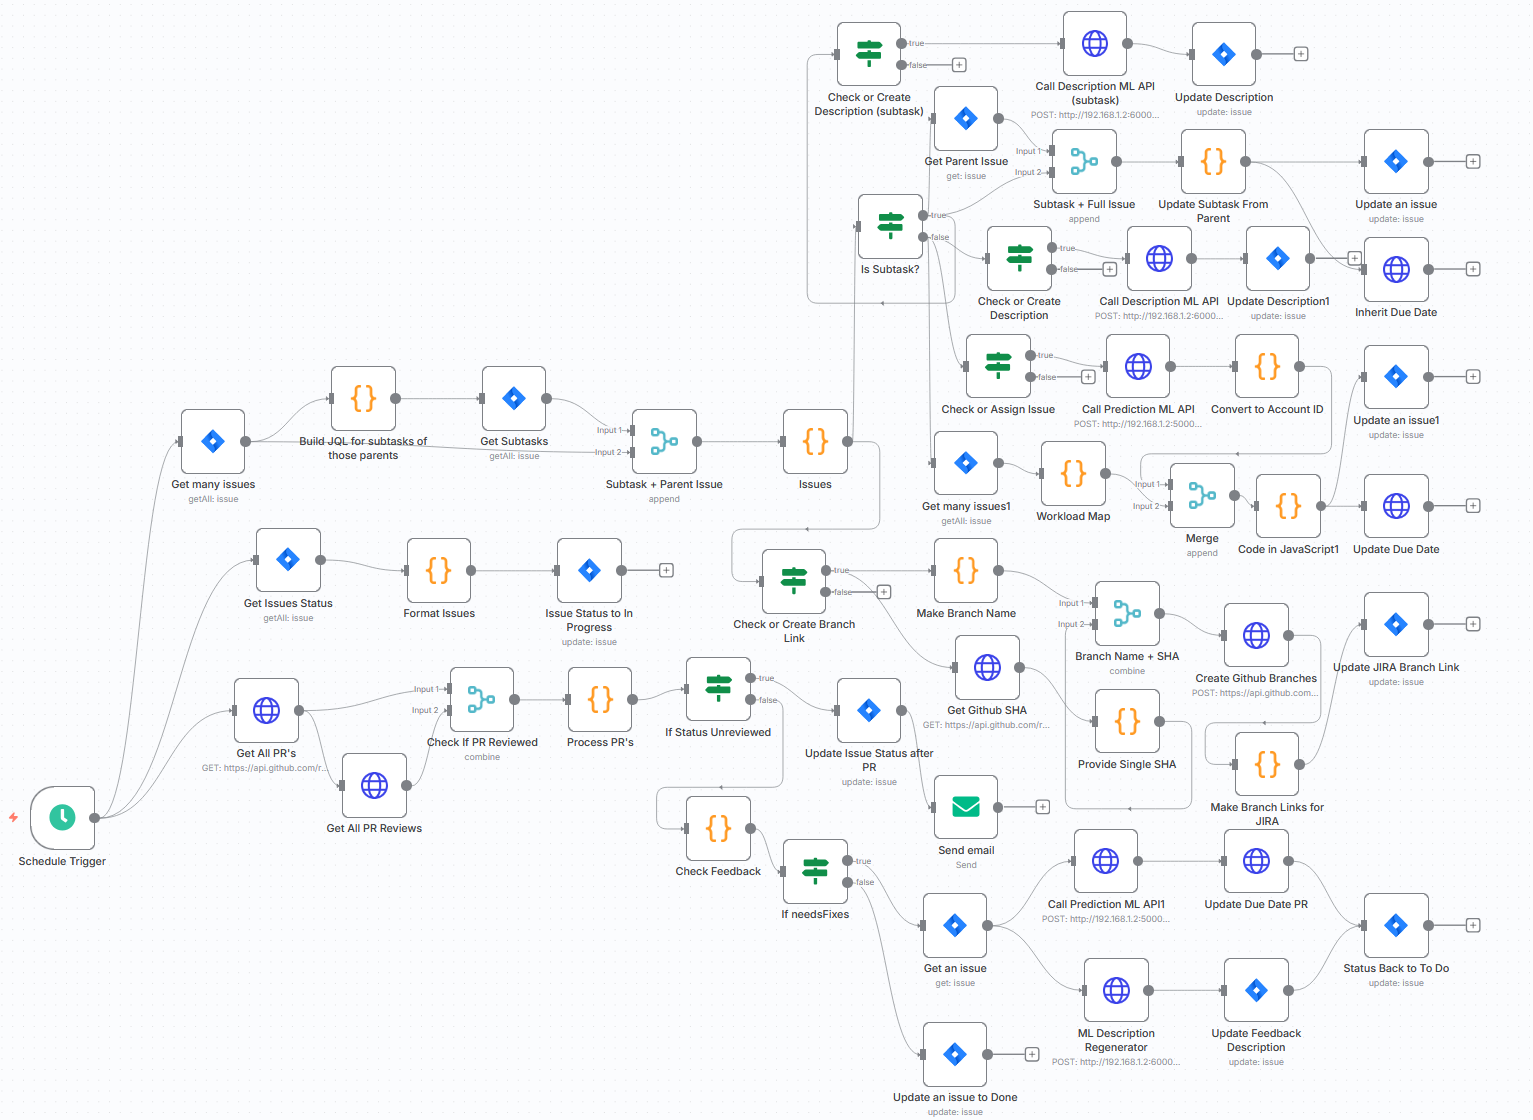
\includegraphics[width=\textwidth]{figures/n8n_flow.png}
\caption{n8n workflow for automated task assignment, deadline prediction, pull request monitoring, and iterative sprint re-evaluation.}
\label{fig:n8nflow}
\end{figure*}


% -------------------------------------------------------------
\subsection{Workflow Automation Integration}
% -------------------------------------------------------------

The orchestration layer is implemented in n8n, while Jira acts as the system of record. Fig.~\ref{fig:n8nflow} shows the full workflow design. The automation includes: scheduled re-checks, issue enrichment, prediction calls, Jira field updates, GitHub PR review monitoring, status transitions, and notifications.

\subsubsection{Trigger Mechanisms and Automated Actions}
The workflow is executed using two main trigger patterns:
\begin{itemize}
    \item Scheduled monitoring (bi-daily): periodically fetches active sprint issues, detects incomplete or returned tasks (e.g., missing assignee/due date/description), and re-runs prediction + updates.
    \item PR-driven transitions: reads GitHub pull request and review status to move issues into review/testing, notify reviewers, and return failed items back to To Do with updated feedback-driven descriptions and adjusted due dates.
\end{itemize}

Subtasks are enforced to inherit key fields from the parent issue (assignee and due date) to preserve ownership consistency across decomposition:
\begin{equation}
\mathrm{assignee}(s) \leftarrow \mathrm{assignee}(p),\;\;\;
\mathrm{due}(s) \leftarrow \mathrm{due}(p),
\label{eq:inherit_rule}
\end{equation}
where $p$ is a parent issue and $s$ is its subtask.

\begin{algorithm}[t]
\caption{Automated Task Processing Pipeline}
\label{alg:pipeline}
\begin{algorithmic}[1]
\STATE \textbf{Input:} Jira issue set $\mathcal{I}$ from active sprint, GitHub PR set $\mathcal{P}$
\STATE \textbf{Output:} Updated Jira fields (assignee, due date, description, status)
\FOR{each issue $i \in \mathcal{I}$}
    \IF{$i$ is subtask}
        \STATE fetch parent $p$ and apply Eq.~\eqref{eq:inherit_rule}
    \ENDIF
    \IF{assignee/due/description missing OR $i$ returned from review}
        \STATE call \texttt{/predict/all} with features of $i$
        \STATE update assignee and due date in Jira based on the predicted duration
        \STATE optionally call \texttt{/generate-description} and update description
    \ENDIF
\ENDFOR
\FOR{each PR $p \in \mathcal{P}$}
    \IF{PR opened}
        \STATE move linked issue to Review/Testing and notify reviewer
    \ENDIF
    \IF{PR review failed}
        \STATE move linked issue back to To Do, update description from feedback, revise due date
    \ELSE
        \STATE move linked issue to Done
    \ENDIF
\ENDFOR
\end{algorithmic}
\end{algorithm}

Model retraining is performed offline on accumulated historical data and is not part of the n8n workflow execution. The automation layer exclusively performs inference using fixed model parameters, ensuring predictable latency and stable behavior during sprint execution.

Cold-start scenarios, such as newly introduced developers with no historical records, are handled outside the predictive model using rule-based assignment strategies (e.g., default role ownership or manual assignment) and are excluded from model training and evaluation.


% -------------------------------------------------------------
\subsection{Evaluation Metrics}
% -------------------------------------------------------------

Assignee performance is evaluated using top-$k$ accuracy to reflect recommendation usage, while deadline estimation is evaluated using MAE, MAPE, and $R^2$.

The evaluation protocol follows a stratified train--test split for classification and standard hold-out evaluation for regression on merged multi-project data, consistent with the deployment goal of stable real-time inference.

For assignee prediction, reported performance corresponds to an unseen 20\% hold-out test set to reflect realistic deployment conditions.

% -------------------------------------------------------------
% -------------------------------------------------------------
\section{Results and Discussion}
% -------------------------------------------------------------

This section reports the experimental evaluation of the proposed assignee recommendation and deadline prediction models and discusses implications for embedding inference into an n8n-driven Agile automation pipeline, including model robustness, baseline comparisons, and workflow-level execution aspects.

% -------------------------------------------------------------
\subsection{Experimental Setup}
% -------------------------------------------------------------

\subsubsection{Experimental Environment}
All experiments were executed on a local workstation environment summarized in Table~\ref{tab:exp_env}. The prediction services were deployed as Flask REST endpoints to enable direct invocation from n8n.

\begin{table}[t]
\centering
\caption{Experimental environment (hardware and software).}
\renewcommand{\arraystretch}{1.1}
\begin{tabular}{l l}
\hline
\textbf{Item} & \textbf{Specification} \\
\hline
CPU & AMD Ryzen 9 5900HS \\
GPU & NVIDIA GeForce RTX 3060 Laptop (6GB) \\
RAM & 16 GB \\
OS & Windows 10 (10.0.26200) \\
Python & 3.11.9 \\
Libraries & scikit-learn 1.6.1, xgboost 2.1.3, flask 3.1.0 \\
\hline
\end{tabular}
\label{tab:exp_env}
\end{table}

\subsubsection{Dataset Split and Protocol}
For assignee recommendation (Aurora project), two evaluation views are reported: (i) 5-fold stratified cross-validation to estimate robustness under class imbalance with oversampling applied only inside each training fold, and (ii) an unseen 20\% hold-out test split (165 issues) to reflect deployment conditions. For deadline prediction, evaluation is performed at the sprint level. Resolution times are filtered to a 7--35 day range, yielding 38 clean sprint records. A fixed 80/20 hold-out split is applied at the sprint level (30 training sprints, 8 testing sprints) with random seed 42 to verify generalization on unseen sprints. Reported regression metrics (MAE, MAPE, and $R^2$) are computed on the 8-sprint test set.


\begin{table}[t]
\centering
\caption{Dataset configuration summary.}
\renewcommand{\arraystretch}{1.1}
\begin{tabular}{l l}
\hline
\textbf{Component} & \textbf{Configuration} \\
\hline
Assignee model & Aurora, 8 developers (whitelist), oversampling-only \\
Split (assignee) & Stratified 80/20 train--test (165 test issues) \\
Deadline model & Sprint-level subset (filtered 7--35 days) \\
Split (deadline) & 80/20 by sprint (30 train, 8 test), seed 42 \\
\hline
\end{tabular}
\label{tab:data_cfg}
\end{table}


% -------------------------------------------------------------
% -------------------------------------------------------------
\subsection{Task Assignment Model Evaluation}
% -------------------------------------------------------------

To obtain robust estimates under class imbalance, we performed 5-fold stratified cross-validation with safe oversampling applied within each training fold. Table~\ref{tab:cls_cv} reports the mean accuracy, standard deviation, and 95\% confidence intervals across folds for several classical baselines and NLP-enhanced models. Oversampling is applied only to the training partition in each fold and is never applied to validation or hold-out test data.

\begin{table}[t]
\centering
\caption{Assignee prediction using 5-fold stratified cross-validation (95\% confidence intervals).}
\renewcommand{\arraystretch}{1.1}
\begin{tabular}{l c c c}
\hline
\textbf{Model} & \textbf{Mean Acc.} & \textbf{Std.} & \textbf{95\% CI} \\
\hline
Dummy (Baseline)        & 0.1250 & 0.0168 & [0.1042, 0.1458] \\
Random Forest (NLP)     & 0.7839 & 0.0550 & [0.7156, 0.8522] \\
XGBoost (NLP)           & 0.7851 & 0.0465 & [0.7273, 0.8429] \\
SVM (NLP)               & 0.7766 & 0.0485 & [0.7164, 0.8368] \\
\hline
\end{tabular}
\label{tab:cls_cv}
\end{table}


XGBoost (NLP) achieved the highest mean cross-validated accuracy (78.51\%) and substantially outperformed the dummy baseline. The confidence intervals show limited overlap between the baseline and NLP-based models, indicating a consistent improvement under this evaluation protocol. In addition, the unseen hold-out split confirms that accuracy drops compared to cross-validation estimates, which is expected under deployment-like conditions.

\begin{table}[t]
\centering
\caption{Assignee prediction on an unseen 20\% hold-out test set (deployment simulation).}
\renewcommand{\arraystretch}{1.05}
\begin{tabular}{l c}
\hline
\textbf{Metric} & \textbf{Result} \\
\hline
Top-1 Accuracy & 0.7879 \\
Top-3 Accuracy & 0.9455 \\
Macro F1-score & 0.77 \\
\hline
\end{tabular}
\label{tab:assignee_holdout}
\end{table}



% -------- DROP YOUR IMAGE HERE (Assignee confusion matrix) --------
\begin{figure}[t]
\centering
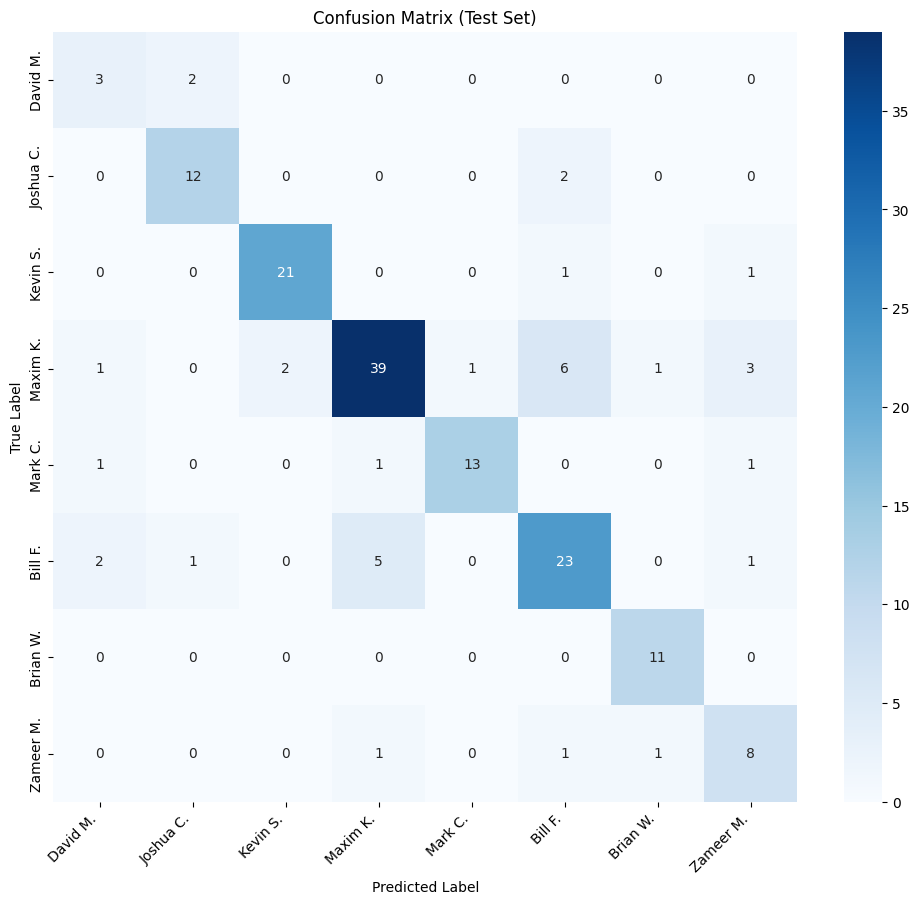
\includegraphics[width=0.6\linewidth]{figures/assignee_confusion_matrix.png}
\caption{Confusion matrix of the assignee recommendation model (XGBoost).}
\label{fig:cm_assignee}
\end{figure}

\subsubsection{Discussion}
Cross-validation results indicate that NLP-enhanced models consistently outperform the dummy baseline, with XGBoost achieving the highest mean accuracy. However, performance on the unseen hold-out split is lower than cross-validation estimates, which is expected under realistic deployment conditions. The hold-out results (Top-1 accuracy of 78.8\%) therefore represent a more conservative and operationally relevant estimate of assignee recommendation performance.





% -------------------------------------------------------------
\subsection{Deadline Prediction Model Evaluation}
% -------------------------------------------------------------

Deadline prediction performance was evaluated using an identical 80/20 hold-out split across all models to ensure a fair comparison. Table~\ref{tab:deadline_baseline} reports mean absolute error (MAE) for each method on the same unseen test set.

\begin{table}[t]
\centering
\caption{Deadline prediction performance on the same unseen test split.}
\renewcommand{\arraystretch}{1.1}
\begin{tabular}{l c}
\hline
\textbf{Model} & \textbf{MAE (days)} \\
\hline
Mean predictor (baseline) & 1.3417 \\
Linear Regression & 1.1124 \\
Random Forest (proposed) & \textbf{0.9157} \\
\hline
\end{tabular}
\label{tab:deadline_baseline}
\end{table}


\subsubsection{Predicted vs. Actual and Residual Behavior}
Fig.~\ref{fig:scatter_deadline} (scatter) and Fig.~\ref{fig:resid_deadline} (residual distribution) are used to inspect calibration and systematic bias.

% -------- DROP YOUR IMAGE HERE (Scatter plot) --------
\begin{figure}[t]
\centering
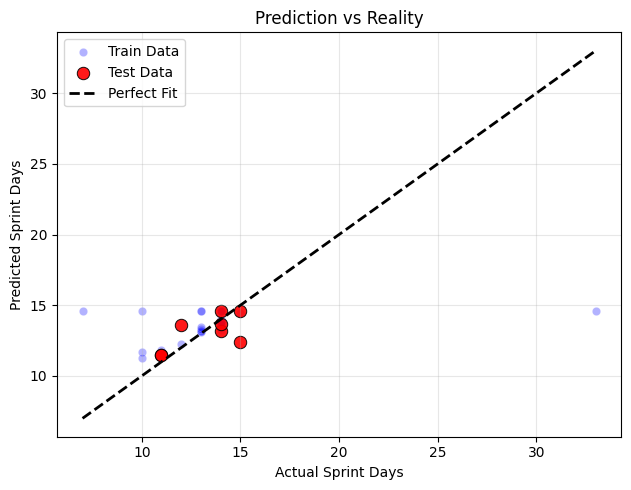
\includegraphics[width=0.6\linewidth]{figures/deadline_scatter.png}
\caption{Predicted vs. actual completion time (days).}
\label{fig:scatter_deadline}
\end{figure}

% -------- DROP YOUR IMAGE HERE (Residuals plot) --------
\begin{figure}[t]
\centering
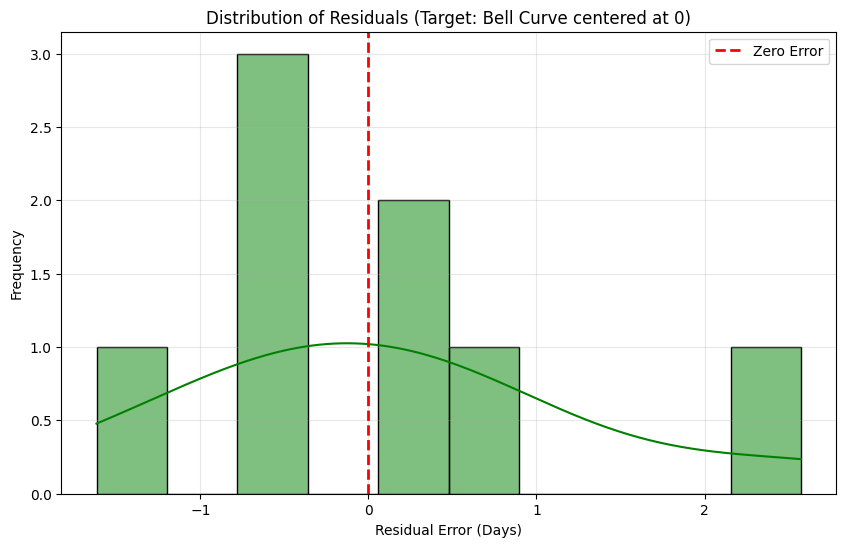
\includegraphics[width=0.6\linewidth]{figures/deadline_residuals.png}
\caption{Residual distribution of the deadline regression model.}
\label{fig:resid_deadline}
\end{figure}

\subsubsection{Discussion (Limitations of Deadline Predictability)}
Although gradient-boosted models such as XGBoost achieved lower error on specific test splits, cross-validation analysis revealed high variance and unstable generalization across folds. In contrast, the Random Forest regressor demonstrated consistently lower MAE across repeated splits and outperformed both the mean and linear regression baselines by a substantial margin. Consequently, model selection prioritized robustness and stability over peak accuracy, aligning with the requirements of reliable sprint-level automation.

Despite improvements in absolute error, the coefficient of determination remains moderate, indicating that a significant portion of variance in issue resolution time is not captured by issue-time features alone. This reflects the influence of latent factors such as scope changes, review delays, and external interruptions, which are unavailable at prediction time. Therefore, deadline prediction is framed as an approximation to support planning rather than a deterministic estimator of completion time.

\begin{table}[t]
\centering
\caption{Regression benchmark across multiple models (illustrative comparison).}
\renewcommand{\arraystretch}{1.05}
\begin{tabular}{l c c c}
\hline
\textbf{Model} & \textbf{MAE} & \textbf{$R^2$} & \textbf{Time (s)} \\
\hline
XGBoost & 0.708 & 0.731 & 0.221 \\
Gradient Boosting & 1.152 & 0.366 & 0.038 \\
Random Forest & 1.224 & 0.276 & 0.135 \\
SVR & 1.258 & 0.154 & 0.005 \\
Neural Network & 1.636 & -0.226 & 0.124 \\
\hline
\end{tabular}
\end{table}

While XGBoost exhibits strong pointwise accuracy, its higher variance across folds motivated the selection of Random Forest for deployment to avoid brittle behavior in production workflows.

Inference latency for the models remained below one second per request in the local environment, which is sufficient for asynchronous workflow execution in n8n. The automation processes issues in batches during scheduled checks, and overall throughput is primarily constrained by external API response times rather than model inference. 

Overall, the results show that combining structured metadata with lightweight text features enables assignee recommendation accuracy close to 80\% on unseen data, substantially exceeding naive baselines. For deadline estimation, the proposed Random Forest model reduces absolute error by approximately 18\% compared to a linear baseline, while maintaining stable behavior under repeated splits. These findings support the feasibility of embedding machine learning inference into Agile workflow automation, provided that predictions are interpreted as decision support rather than exact forecasts.


% -------------------------------------------------------------
\subsection{Baseline Comparison}
% -------------------------------------------------------------

To contextualize regression performance, Table~\ref{tab:deadline_baseline} compares the proposed deadline model against a simple mean predictor baseline. The proposed model reduces MAE by 17.7\% compared to the linear regression baseline (1.1124 to 0.9157 days) and by 31.8\% compared to the mean predictor (1.3417 to 0.9157 days) on the same unseen test split.

% -------------------------------------------------------------
\subsection{System Integration Performance}
% -------------------------------------------------------------

\subsubsection{End-to-end Orchestration in n8n}
The deployed Flask endpoint \texttt{/predict/all} is invoked from n8n to obtain both assignee recommendations and predicted deadline days, which are then written back to Jira fields. The workflow also includes workload-aware selection from top-$k$ candidates and automated due date updates.

\subsubsection{Scheduling and Continuous Monitoring}
The workflow is triggered periodically using a schedule trigger (bi-daily re-check design), enabling continuous re-evaluation of issues that are incomplete (missing assignee/due date/description) or returned from review. The schedule-trigger mechanism is supported directly by n8n core nodes.

% -------------------------------------------------------------
\subsection{Discussion}
% -------------------------------------------------------------

Overall, the experiments indicate that combining lightweight structured metadata with TF--IDF text features enables assignee recommendation performance beyond naive baselines (cross-validated accuracy around 0.79; hold-out Top-1 accuracy 0.79). For deadline estimation, the tuned model yields low absolute error (MAE below one day) while achieving moderate explained variance, reflecting the inherent uncertainty of completion time. These findings align with prior work that uses issue metadata for operational decision support \cite{razi2023_projectml}, while emphasizing the need for cautious interpretation of deadline predictability.

\subsubsection{Threats to Validity and Limitations}
Several limitations should be considered. First, the assignee model is trained on a single project subset (Aurora) and evaluated under oversampling-only balancing, which can inflate measured performance relative to real-world imbalanced distributions. Second, the deadline model uses a compact feature set, incorporating richer signals (e.g., PR review duration, dependency links, developer availability, or historical cycle time per component) may improve $R^2$ but increases integration complexity. Third, results are based on Jira like open-source data and may not transfer directly to proprietary enterprise workflows without re-training and schema alignment.

\subsubsection{Practical Implications}
Despite these limitations, embedding ML inference into a workflow engine provides immediate operational value: it reduces manual triage overhead, enforces completeness constraints, and standardizes how tasks progress across sprint phases. In practice, adopting top-$k$ recommendations plus workload constraints in n8n offers a robust compromise between model uncertainty and real-world resource management.

\begin{table}[t]
\centering
\caption{Per-class performance of the assignee model on the hold-out test set (165 issues).}
\renewcommand{\arraystretch}{1.05}
\begin{tabular}{l c c c}
\hline
\textbf{Class} & \textbf{Prec.} & \textbf{Rec.} & \textbf{F1} \\
\hline
David M.  & 0.43 & 0.60 & 0.50 \\
Joshua C. & 0.80 & 0.86 & 0.83 \\
Kevin S.  & 0.91 & 0.91 & 0.91 \\
Maxim K.  & 0.85 & 0.74 & 0.79 \\
Mark C.   & 0.93 & 0.81 & 0.87 \\
Bill F.   & 0.70 & 0.72 & 0.71 \\
Brian W.  & 0.85 & 1.00 & 0.92 \\
Zameer M. & 0.57 & 0.73 & 0.64 \\
\hline
\end{tabular}
\label{tab:assignee_perclass}
\end{table}

% -------------------------------------------------------------
% -------------------------------------------------------------
\section{Conclusion}
% -------------------------------------------------------------

This study examined the feasibility of embedding machine learning inference into an automated Agile project management workflow to reduce manual coordination overhead during sprint execution. The proposed system integrates supervised learning for assignee recommendation and regression-based deadline estimation, deployed as RESTful services and orchestrated through an n8n automation pipeline connected to Jira-like issue trackers. Rather than introducing novel algorithms, the contribution focuses on operationalizing predictive models within a live workflow environment.

Experimental results show that the assignee recommendation model achieves a Top-1 accuracy of 78.8\% and a Top-3 accuracy of 94.5\% on an unseen hold-out test set, substantially outperforming naive baselines. These results indicate that combining lightweight textual features with structured issue metadata is effective for recommendation-based task assignment under realistic deployment conditions. Cross-validation further confirms that the selected model exhibits stable performance across multiple data splits.

For deadline estimation, the proposed Random Forest regressor reduces mean absolute error by approximately 18\% compared to a linear regression baseline on the same unseen test set. However, the coefficient of determination remains modest, indicating that a large portion of variance in issue resolution time cannot be explained by issue-time features alone. This outcome highlights the inherently stochastic nature of Agile development, where factors such as scope changes, review delays, and external interruptions are not observable at prediction time. Consequently, deadline predictions should be interpreted as coarse guidance rather than precise forecasts.

The primary contribution of this work lies in demonstrating how machine learning models can be reliably integrated into an automated workflow engine to support consistent task handling during sprint execution. By embedding inference into n8n orchestration, the system enables automated assignment, due-date suggestion, and periodic re-evaluation of incomplete or returned issues without relying on continuous model retraining. This workflow-centric perspective distinguishes the approach from prior studies that focus primarily on offline prediction accuracy.

Future work will focus on improving deadline estimation robustness by incorporating additional process-level signals that are available during sprint execution, such as pull request activity, review duration, or historical cycle time at the component level. Further evaluation on larger and proprietary datasets is also required to assess generalizability across organizational contexts. Overall, this study demonstrates that modest but stable predictive models, when tightly coupled with workflow automation, can provide meaningful decision support in Agile project management without over-relying on complex or opaque modeling techniques.




\begin{thebibliography}{00}

\bibitem{verwijs2023_scrum}
C. Verwijs and D. Russo, ``A Theory of Scrum Team Effectiveness,''
\textit{ACM Trans. Softw. Eng. Methodol.}, vol. 32, no. 3, Art. 74, Apr. 2023,
doi: 10.1145/3571849.

\bibitem{gemino2021_project_success}
A. Gemino, B. H. Reich, and R. Serrador, ``Agile, traditional, and hybrid approaches to project success: Is hybrid a poor second choice?''
\textit{Project Management Journal}, vol. 52, no. 2, pp. 161--175, 2021,
doi: 10.1177/8756972820973082.

\bibitem{gibbs2023_wfh_productivity}
M. Gibbs, F. Mengel, and C. Siemroth, ``Work from Home and Productivity: Evidence from Personnel and Analytics Data on IT Professionals,''
\textit{J. Political Economy Microeconomics}, vol. 1, no. 2, pp. 235--275, 2023,
doi: 10.1086/721803.

\bibitem{venkatesh2020_work_exhaustion}
V. Venkatesh, J. Y. L. Thong, and F. K. Y. Chan, ``How Agile Software Development Methods Reduce Work Exhaustion: Insights on Role Perceptions and Organizational Skills,''
\textit{Information Systems Journal}, vol. 30, no. 5, pp. 829--859, 2020,
doi: 10.1111/isj.12282.

\bibitem{prinz2021_lowcode_slr}
N. Prinz, C. Rentrop, and M. Huber, ``Low-Code Development Platforms -- A Literature Review,''
in \textit{Proc. Americas Conf. Inf. Syst. (AMCIS)}, 2021.

\bibitem{gupta2023_action_suggestions}
S. Gupta \textit{et al.}, ``Personalized Action Suggestions in Low-Code Automation Platforms,''
in \textit{Proc. IEEE/ACM Int. Conf. Softw. Eng. Companion (ICSE-Companion)}, 2023,
doi: 10.1109/ICSE-Companion58688.2023.00100.

\bibitem{zhao2021_trigger_action}
D. Zhao \textit{et al.}, ``What Can We Learn from a Dataset of If-This-Then-That Recipes?''
in \textit{Proc. CHI Conf. Human Factors in Computing Systems (CHI)}, 2021,
doi: 10.1145/3411764.3445567.

\bibitem{yusuf2022_tap_generation}
D. M. Yusuf \textit{et al.}, ``Accurate and Complete Generation of Trigger-Action Programs from Natural Language Instructions Using a Domain-Adapted Seq2Seq Model,''
in \textit{Proc. IEEE/ACM Int. Conf. Program Comprehension (ICPC)}, 2022.

\bibitem{yasmin2024_airflow_wac}
J. Yasmin, J. Wang, Y. Tian, and B. Adams, ``An Empirical Study of Developers' Challenges in Implementing Workflows as Code: A Case Study on Apache Airflow,''
\textit{arXiv preprint} arXiv:2406.00180, 2024.

\bibitem{shamim2025_costreview}
M. M. I. Shamim, A. B. A. Hamid, T. E. Nyamasvisva, and N. S. B. Rafi,
``Advancement of Artificial Intelligence in Cost Estimation for Project Management Success: A Systematic Review of Machine Learning, Deep Learning, Regression, and Hybrid Models,''
\textit{Modelling}, vol. 6, no. 2, Art. 35, 2025,
doi: 10.3390/modelling6020035.

\bibitem{mahdi2021_spm_slr}
N. Mahdi \textit{et al.}, ``Machine Learning for Software Project Management: A Systematic Literature Review,''
\textit{Applied Sciences}, vol. 11, no. 23, 2021.

\bibitem{cabral2023_ensemble_effort}
J. T. H. d. A. Cabral, R. Gomes, and A. Mendes-Moreira,
``Ensemble Effort Estimation: An Updated and Extended Systematic Literature Review,''
\textit{J. Syst. Softw.}, vol. 195, Art. 111542, 2023,
doi: 10.1016/j.jss.2022.111542.

\bibitem{sousa2023_task_effort}
T. Sousa \textit{et al.}, ``Applying Machine Learning to Estimate the Effort and Duration of Individual Tasks in Software Projects,''
\textit{IEEE Access}, vol. 11, pp. 89933--89946, 2023,
doi: 10.1109/ACCESS.2023.3287537.

\bibitem{mahmud2022_risk_slr}
M. S. Mahmud \textit{et al.}, ``Software Project Risk Prediction Using Machine Learning: A Systematic Literature Review,''
\textit{Applied Sciences}, vol. 12, no. 4, 2022.

\bibitem{perezcastillo2024_sprint_velocity}
Y. J. P\'erez Castillo, S. D. Orantes Jim\'enez, and P. O. Letelier Torres,
``Sprint Management in Agile Approach: Progress and Velocity Evaluation Applying Machine Learning,''
\textit{Information}, vol. 15, no. 11, Art. 726, 2024,
doi: 10.3390/info15110726.

\bibitem{ramessur2021_sprint_effort}
S. Ramessur and S. D. Nagowah,
``Software Effort Estimation in a Sprint Using Machine Learning Regression Techniques,''
\textit{Int. J. Inf. Technol.}, vol. 13, pp. 1--10, 2021,
doi: 10.1007/s41870-021-00669-z.

\bibitem{yalciner2024_storypoint_sbert}
B. Yal\c{c}{\i}ner and D. Baturay,
``Enhancing Agile Story Point Estimation: Integrating Deep Learning, Machine Learning, and Natural Language Processing with SBERT and Gradient Boosted Trees,''
\textit{Applied Sciences}, vol. 14, no. 16, Art. 7305, 2024,
doi: 10.3390/app14167305.

\bibitem{choetkiertikul2025_sprint2vec}
M. Choetkiertikul \textit{et al.},
``Sprint2Vec: A Deep Characterization of Sprints in Iterative Software Development,''
\textit{IEEE Trans. Softw. Eng.}, vol. 51, no. 1, pp. 220--242, 2025,
doi: 10.1109/TSE.2024.3509016.

\bibitem{diamantopoulos2023_issue_assignment}
T. Diamantopoulos, N. Saoulidis, and A. Symeonidis,
``Automated Issue Assignment Using Topic Modelling on Jira Issue Tracking Data,''
\textit{IET Software}, vol. 17, no. 3, pp. 333--344, 2023,
doi: 10.1049/sfw2.12129.

\bibitem{nastos2025_resolution_time}
D.-N. Nastos, T. Diamantopoulos, D. Tosi, M. Tropeano, and A. Symeonidis,
``Towards an Interpretable Analysis for Estimating the Resolution Time of Software Issues,''
\textit{arXiv preprint} arXiv:2505.01108, 2025.

% (Fixed: broken quotes/backticks + "Proc. IEEE" misuse)
\bibitem{brar2022_effort_slr}
A. Brar and A. Nandal,
``A Systematic Literature Review on Software Effort Estimation Using Machine Learning Techniques,''
in \textit{Proc. (IEEE-indexed) Conf.}, 2022.

\bibitem{guo2020_bug_triage}
S. Guo \textit{et al.}, ``Developer Activity Motivated Bug Triaging: Via Convolutional Neural Network,''
\textit{Neural Process. Lett.}, vol. 52, pp. 1--18, 2020,
doi: 10.1007/s11063-020-10213-y.

\bibitem{zhang2023_susrec}
W. Zhang, J. Zhao, R. Peng, S. Wang, and Y. Yang,
``SusRec: An Approach to Sustainable Developer Recommendation for Bug Resolution Using Multimodal Ensemble Learning,''
\textit{IEEE Trans. Reliability}, vol. 72, no. 1, pp. 61--78, 2023,
doi: 10.1109/TR.2022.3176733.

\bibitem{kaur2023_agile_resource_alloc}
H. Kaur, D. P. Kaur, and K. S. S. Kaler,
``An Agile-Based Software Development Resource Allocation Approach with Multi-Objective Goal Programming,''
\textit{Digital Applications}, 2023,
doi: 10.1016/j.dajour.2022.100146.

\bibitem{cai2024_drl_rcpsp}
Y. Cai \textit{et al.}, ``Deep Reinforcement Learning for the Resource-Constrained Project Scheduling Problem,''
\textit{IEEE Trans. Autom. Sci. Eng.}, 2024.

\bibitem{koralage2023_velocity}
R. U. Koralage, ``Novel Approach to Estimate Velocity for Agile Scrum Sprint Planning,''
Preprint, Dec. 2023, doi: 10.13140/RG.2.2.17595.18721.

\bibitem{teguh2023_mlworkflow}
A. Teguh, R. Widyastuti, and H. Prasetyo,
``Machine Learning-Based Task Management for Software Project Workflows,''
in \textit{Proc. IEEE Int. Conf. on Information Technology Systems and Innovation (ICITSI)}, 2023, pp. 1--6.

\bibitem{razi2023_projectml}
M. Razi, A. F. Ramadhan, and S. Hidayat,
``Applying Machine Learning for Decision Support in Software Project Management,''
in \textit{Proc. IEEE Int. Conf. on Advanced Computer Science and Information Systems (ICACSIS)}, 2023, pp. 1--6.

\bibitem{alekhine2024_jira}
J. Alekhine \textit{et al.}, ``Project Management Ticket Category Classification using Machine Learning Method: A Comparative Study,''
in \textit{Proc. IEEE Int. Conf. Artificial Intelligence and Mechatronics Systems (AIMS)}, 2024.

\bibitem{automl_se_slr}
M. A. Ahmed, M. J. Shepperd, and S. Counsell,
``AutoML for Software Engineering: A Systematic Literature Review,''
\textit{IEEE Trans. Softw. Eng.}, 2022.



\end{thebibliography}




\end{document}
